% document formatting
\documentclass[10pt]{article}
\usepackage[utf8]{inputenc}
\usepackage[left=1in,right=1in,top=1in,bottom=1in]{geometry}
\usepackage[T1]{fontenc}
\usepackage{xcolor}

% math symbols, etc.
\usepackage{amsmath, amsfonts, amssymb, amsthm}

% lists
\usepackage{enumerate}

% images
\usepackage{graphicx} % for images

% code blocks
\usepackage{minted, listings} 

% verbatim greek
\usepackage{alphabeta}

\graphicspath{{./assets/images}}

\newcommand{\solution}{\textbf{Solution:}} 

\title{COM SCI M151B Week 2}

\author{Aidan Jan}
\date{\today}

\begin{document}
\section*{Microarchitecture}
\begin{itemize}
    \item The hardware implementation of ISA is called \textit{microarchitecture}
    \item A given ISA (e.g., RISC-V) can be implemented in many different ways (i.e., same ISA, different microarchitecture)
    \item The goal is to build an \textit{efficient} computer
    \begin{itemize}
        \item Fast (high performance) and power efficient.
    \end{itemize}
\end{itemize}

\subsection*{State-Machine View}
\begin{itemize}
    \item How do we make a microarchitecture?  
    \item There are two different parts:
    \begin{enumerate}
        \item Controller: a unit that directs the operation/activities on the datapath
        \item Data Path: a collection of \textit{functional} units that process the data and create the data-flow
    \end{enumerate}
\end{itemize}
\begin{center}
    \includegraphics*[scale=0.8]{W2_1.png}
    \includegraphics*[scale=0.8]{W2_2.png}
\end{center}
We will go through how this works, step by step.  But first, how are instructions executed?
\subsection*{Lifecycle of an instruction}
\begin{enumerate}
    \item Instruction is read (fetch) from the (instruction) memory
    \item Operands should be loaded
    \begin{itemize}
        \item RegFile, (data) Memory, Immediates
        \item Need register number / address for each operand
    \end{itemize}
    \item Operation should be executed
    \begin{itemize}
        \item Arithmetic (which type?), data movement, control-flow.
    \end{itemize}
    \item Results should be stored
    \begin{itemize}
        \item RegFile or memory?
    \end{itemize}
    \item PC should be updated
    \begin{itemize}
        \item Usually it is PC += 4, but sometimes it is different due to jumping/branching.
    \end{itemize}
\end{enumerate}
\subsubsection*{Instruction Fetch}
Provide a read address to the instruction, and get a 32 bit instruction.
\begin{center}
\includegraphics*[scale=0.8]{W2_3.png}
\end{center}
Registers stores data in a circuit. 
\begin{itemize}
    \item Uses a clock signal to determine when to update the stored value (could be multiple bits).
    \item Data stored in a register is read/written on the positive edge of the clock cycle.
    \item Uses D-flip-flop
    \item Some registers have a write-enable input.  If this is present, memory is only written when control input is 1.
\end{itemize}
Memory is an \textit{array of registers}.
\begin{itemize}
    \item Specific line can be chosen via a multiplexer.
\end{itemize}
\subsubsection*{Memory Technology}
\begin{itemize}
    \item Are all memory cells registers, SRAM, DRAM, etc.?
    \item No!
    \item \textbf{Latches and Flip-Flops (aka Registers)}
    \begin{itemize}
        \item Very fast (1 cycle), parallel access.
        \item Very expensive (one bit costs tens of transistors).
    \end{itemize}
    \item \textbf{Static RAM (SRAM)}
    \begin{itemize}
        \item Relatively fast (10 cycles), only one data word at a time.
        \item Expensive (one bit costs 6+ transistors).
    \end{itemize}
    \item \textbf{Dynamic RAM (DRAM)}
    \begin{itemize}
        \item Slower (100 cycles), one data word at a time, reading \textit{destroys} content (refresh), needs special process for manufacturing
        \item Cheap (one bit costs only one transistor plus one capacitor).
    \end{itemize}
    \item \textbf{DISK}
    \begin{itemize}
        \item flash memory, hard disk
        \item Much slower (1000+ cycles), access takes a long time
        \item Non-volatile
        \item Very cheap
    \end{itemize}
\end{itemize}
Which type of storage should we use?
\begin{itemize}
    \item From Register to DRAM to disk:
    \begin{itemize}
        \item From \textit{smaller} and \textit{faster} $\rightarrow$ \textit{bigger} and \textit{slower}
        \item From \textit{more expensive} and \textit{power hungry} $\rightarrow$ \textit{cheaper} and \textit{power efficient}
        \item The type we need depends on the purpose we need it for.  Use registers for frequently used data and slower and bigger elements for rarely-used permanent data.
    \end{itemize}
\end{itemize}
\subsubsection*{Loading Operands}
\begin{itemize}
    \item To load values from registers, we provide an address to read, with the write data bit at 0.  
    \item To write, we provide an address, the data to write, and the write enable bit.
    \item However, \textit{how could we know which instruction we read?}
    \begin{itemize}
        \item We need a controller!
    \end{itemize}
\end{itemize}
\begin{center}
    \includegraphics*[scale=0.5]{W2_4.png}
\end{center}
The controller directs the operations for each instruction.
\begin{center}
    \includegraphics*[scale=0.6]{W2_5.png}
\end{center}
We build controllers using finite state machines (FSMs).

\subsubsection*{Finite-State Machine (FSM)}
\begin{itemize}
    \item A \textit{mathematical} model of computation
    \item At each point, the system can be \textit{only at one} of the several, but \textbf{finite} states.
    \item FSM shows all the states and how they transit to each other.
    \item FSM also includes finite number of inputs and outputs.
\end{itemize}
\begin{center}
    \includegraphics*[scale=0.5]{W2_6.png}
    Remember these from CS181?
\end{center}
The FSM/Controller for a processor is simply a giant FSM with many states!
\begin{itemize}
    \item Lifecycle of each instructon in the controller:
    \begin{itemize}
        \item \textit{Initial State:} reading the instruction and decoding it.
        \item \textit{Next State:} each instruction has its own state.
        \item \textit{Future State:} depending on the instruction, there could be several states (e.g., reading registers, loading memory, arithmetic operations, etc.)
    \end{itemize}
    \item Once all the activities are done, the controller should go back to the \textit{initial state} and \textit{repeat} this process for the next instruction.
    \begin{itemize}
        \item We call this single-cycle design!
    \end{itemize}
\end{itemize}
\subsection*{Building a Simple CPU}
\begin{itemize}
    \item RISC-V ISA, 32-bit
    \item Handful of instructions - only 10
    \begin{itemize}        
        \item add, sub, and, or, lw, sw, beq, addi, andi, ori
    \end{itemize}
\end{itemize}
\subsubsection*{Creating nextPC}
Implement the part where you increment the program counter by 4.
\begin{center}
    \includegraphics*[scale=0.4]{W2_7.png}
\end{center}
\begin{itemize}
    \item Note that this will be modified later since we have branching, and not every instruction will increment by 4!
\end{itemize}
\subsubsection*{ALU}
\begin{center}
    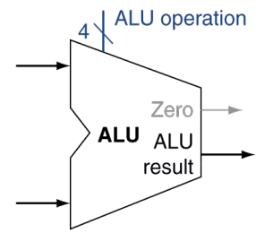
\includegraphics[scale=0.8]{W2_8.png}
\end{center}
ALU has two 32-bit inputs, an ALU result and Zero (x0) output, as well as a ALU operation with 4 bits, which selects the ALU operation to execute.
\subsubsection*{Register to ALU}
We need to connect the registers to the ALU.
\begin{center}
    \includegraphics*[scale=0.6]{W2_9.png}
\end{center}
\begin{itemize}
    \item The Immediate Generator takes in the bits of the instruction and shuffles it with the immediates to get the correct instruction format.  (funct7, rs2, rs1, funct3, rd, opcode, etc.)  Also does zero-padding if necessary.
    \item The registers provides the values in the registers that are needed.
    \item For R-type instructions without the need of immediates, the immediate generator generates garbage.  However, it does not matter since the MUX will not select it for the ALU.
\end{itemize}
\subsubsection*{Putting it all together}
\begin{center}
    \includegraphics*[scale=0.7]{W2_10.png}
\end{center}
The MemtoReg multiplexer decides whether data should be written.


\end{document}